\documentclass[tikz,border=10pt]{standalone}
\usepackage{tikz}
\usepackage{amsmath}
\usepackage{xcolor}

% Define colors
\definecolor{myred}{RGB}{220,20,60}
\definecolor{myblue}{RGB}{0,100,200}

% TikZ styles for consistency
\tikzset{
    bell curve/.style={thick, smooth, domain=-1:1},
    explanation text/.style={text width=6cm, align=center, font=\small},
    curved arrow/.style={->, thick, bend left=#1},
    math var/.style={font=\normalsize}
}

\begin{document}
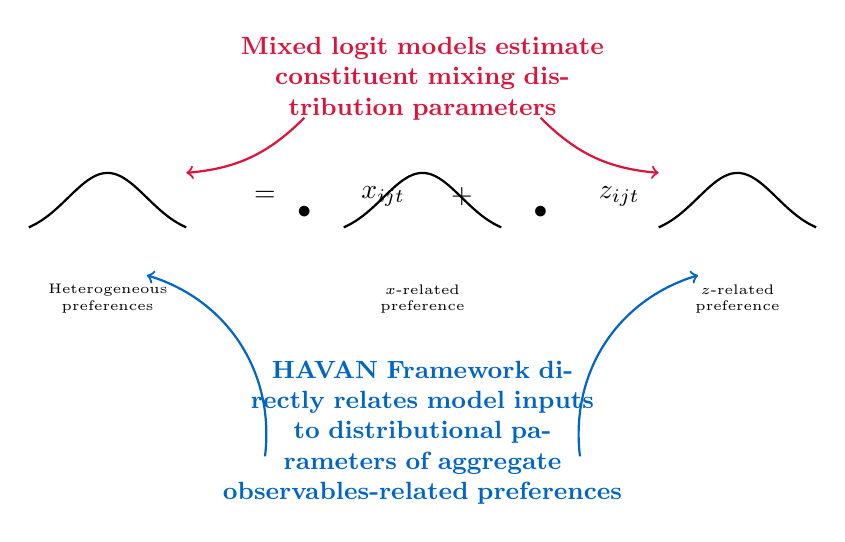
\begin{tikzpicture}[scale=1.0]

% Top explanatory text
\node[explanation text, color=myred] at (0,4) {
    \textbf{Mixed logit models estimate\\
    constituent mixing distribution parameters}
};

% Bell curves
\draw[bell curve] plot ({-4+\x}, {2+0.8*exp(-2*\x*\x)});
\draw[bell curve] plot ({0+\x}, {2+0.8*exp(-2*\x*\x)});
\draw[bell curve] plot ({4+\x}, {2+0.8*exp(-2*\x*\x)});

% Labels under curves
\node[font=\tiny, text width=1.5cm, align=center] at (-4,1.2) {Heterogeneous\\preferences};
\node[font=\tiny, text width=1.5cm, align=center] at (0,1.2) {$x$-related\\preference};
\node[font=\tiny, text width=1.5cm, align=center] at (4,1.2) {$z$-related\\preference};

% Mathematical operations
\node at (-2,2.5) {$=$};
\node at (-1.5,2.3) {$\bullet$};
\node[math var] at (-0.5,2.5) {$x_{ijt}$};
\node at (0.5,2.5) {$+$};
\node at (1.5,2.3) {$\bullet$};
\node[math var] at (2.5,2.5) {$z_{ijt}$};

% Curved arrows from top text
\draw[curved arrow=20, myred] (-1.5,3.5) to (-3,2.8);
\draw[curved arrow=-20, myred] (1.5,3.5) to (3,2.8);

% Bottom explanatory text
\node[explanation text, color=myblue, font=\small] at (0,-0.5) {
    \textbf{HAVAN Framework directly relates model inputs\\
    to distributional parameters of aggregate observables-related preferences}
};

% Curved arrows from bottom text
\draw[curved arrow=-40, myblue] (-2,-0.8) to (-3.5,1.5);
\draw[curved arrow=40, myblue] (2,-0.8) to (3.5,1.5);

\end{tikzpicture}
\end{document}